\documentclass[a4paper, 10pt, twocolumn]{jarticle}
\pagestyle{empty}

\usepackage[dvipdfmx]{graphicx}
\usepackage[top=20truemm, bottom=20truemm, left=18truemm, right=18truemm]{geometry}
\usepackage{calc}
\usepackage{titlesec}
\usepackage{amsmath}
\usepackage[hang,bf]{caption}

\setlength{\columnsep}{\columnsep + 4zw}
\setlength{\textheight}{49\baselineskip}
\titleformat*{\section}{\normalsize\bfseries}
\titleformat*{\subsection}{\normalsize\bfseries}

\titlespacing{\section}{0pt}{4pt}{4pt}
\titlespacing{\subsection}{0pt}{4pt}{4pt}
\setlength{\intextsep}{10pt}
\setlength{\textfloatsep}{10pt}

\linespread{0.81} 


\begin{document}
\twocolumn
[
    \centering
    \vspace{0.5\baselineskip}
    {\large\bfseries
        様々な環境や状況に対応できるPDRベースの3次元屋内位置推定ライブラリに関する研究
    } \\
    \vspace{0.5\baselineskip}
    B23714 外山瑠起 指導教員 梶克彦 \\
    \vspace{\baselineskip}
    キーワード: 屋内位置推定,PDR,ソフトウェアライブラリ

    \vspace{\baselineskip}
    \vspace{\baselineskip}
]


\section{はじめに}


屋内環境における位置推定は,様々なサービスや業務の基盤として重要性を増している.
大規模商業施設での顧客誘導,物流倉庫での作業効率化など,その応用範囲は広がり続けている.
しかし屋内ではGPSなどの衛星測位システムの利用が難しく,代替となる位置推定手法が必要とされる.

% TODO: IMUの所の文章少し違和感
% TODO: 設計されており→されておりでもよさそう
屋内位置推定手法は主に絶対位置推定と相対位置推定に大別される.
絶対位置推定は空間内での絶対的な位置を求める手法であり,
代表的な手法としてWi-FiやBLEなどの電波を用いた手法がある.
相対位置推定は特定の基準点からの相対的な位置を求める手法であり,
代表的な手法であるPDR(歩行者自律航法)は,IMU(慣性計測装置)から得られる加速度と角速度を用いて歩行者の位置を推定する.
近年ではPDRと電波強度を組み合わせた手法\cite{pdr-rss-fusion}や,
フロアマップ情報を活用したマップマッチング手法\cite{pdr-map}など,
複数の手法を統合したアプローチが提案されている.
しかしこれらの手法の多くは特定の環境を想定して設計されており,
異なる環境への部分的な適用は困難である.

そこで本研究では様々な環境や状況に対応可能な,PDRベースの3次元屋内位置推定ライブラリの開発を目的とする.
図1に本研究で提案するライブラリの概要を示す.
本ライブラリはPDRを基盤とし,環境情報を活用した段階的な補正アプローチを導入する.
また拡張性と再利用性を重視したソフトウェアアーキテクチャを採用し,
新たな補正アルゴリズムの追加や既存アルゴリズムの組み合わせを容易にする.


% TODO: 図1が昔に作成したものだから文章とあってない気がする.
\begin{figure}[h]
	\centering
	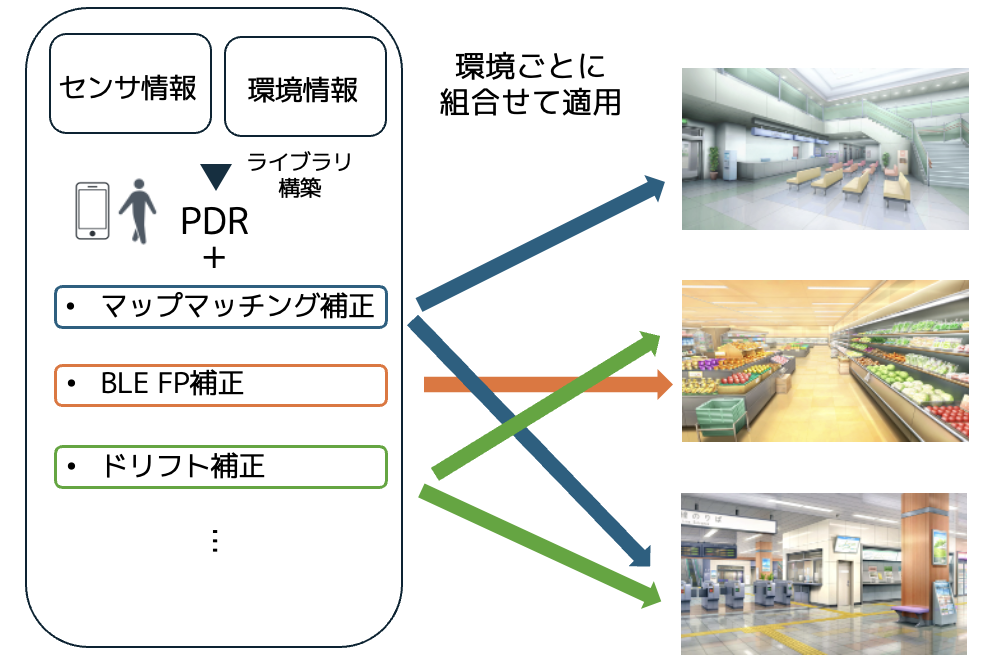
\includegraphics[width=\linewidth]{image/first.png}
  % TODO: captionの文字を中央にできないか検討したい
	\caption{様々な環境や状況に対応できるPDRベースの3次元屋内位置推定ライブラリの概要}    \label{fig:overview}
\end{figure}


\section{PDRベースの3次元屋内位置推定ライブラリの検討}
本章ではPDRベースの3次元屋内位置推定ライブラリの設計と実装について述べる.
要求仕様を整理し,PDRを基盤とした平面的な位置推定手法の実装について説明する.
さらに気圧センサを活用した3次元的な位置推定手法について述べる.


% TODO: 基本が連続して続く
\subsection{要求仕様}
屋内環境における位置推定システムの開発には,
環境条件と利用可能な補正情報の多様性を考慮する必要がある.
本ライブラリでは基本となるセンサ情報として加速度センサとジャイロセンサをPDRの基本処理に,
気圧センサを階層判定による3次元位置推定に利用する.
環境情報としては歩行可能領域の制約として機能するフロアマップ情報と,
位置推定の補正に柔軟に活用できる電波強度情報を採用する.
システムの設計においては補正アルゴリズムを独立したモジュールとして実装し,
環境に応じて適切な組み合わせが可能な設計とする.


% TODO:本システムなのか本ライブラリなのか統一した方がよさそう
% TODO: 選択的という表現が少しくどいか?
\subsection{平面的な位置推定}
本ライブラリではPDREstimatorを中心として,
StepEstimator,OrientationEstimator,TrajectoryCalculatorの3つの主要なクラスが連携して位置推定を行う.
またセンサデータの管理はSensorDataクラスが担当する.
StepEstimatorは加速度信号の変動パターンから歩行動作を検出し,歩行タイミングと歩幅を推定する.
OrientationEstimatorは角速度の積分による方向推定を行う.
TrajectoryCalculatorは推定された歩幅,歩行タイミング,方向から実際の移動軌跡を計算する.

補正処理はTrajectoryCorrectrorクラスを中心とした設計を採用している.
このクラスはDriftCorrector,MapMatchCorrector,WirelessSignalCorrectorの3つの補正クラスを統合的に管理し,
それぞれが特定の補正機能を担当する.各補正クラスは独立したモジュールとして実装され,新しい補正手法の追加時に
既存の処理に影響を与えない.またビルダーパターンを採用し,with\_floor\_map()やwith\_wireless\_signal()などの
メソッドチェーンにより,補正手法の直感的な組み立てと適用順序の制御を行う.

図2に示すように初期軌跡に対して環境条件に応じた補正を選択的に適用できる.
既知の座標が利用可能な場合は,センサの累積誤差を低減するドリフト補正が適用できる.
フロアマップ情報が利用可能な場合は建物の構造的特徴を活用して初期進行方向を補正し,
さらに歩行可能領域の情報から軌跡を補正できる.
Wi-FiやBLEなどの電波強度情報が利用可能な場合は2つのアプローチのうちどちらかを適用できる.
1つは送信機の基地局位置を既知とし,受信強度の閾値処理と距離の最適化により軌跡を補正する手法である.
もう1つはフィンガープリントを用いた手法である.フィンガープリント手法は事前に収集した電波強度パターンと
実測値の類似度に基づいて位置を推定するため,基地局位置が未知の環境でも適用可能な利点がある.


% TODO: 実現するより行うの方がいい?
% TODO: 環境情報と環境条件どちらがいいのか?(統一が大事)
これらの補正手法は環境に応じて選択的に統合適用も可能である.例えば
フロアマップと電波強度情報の両方が利用可能な環境では,まず建物の構造を考慮した補正を行う.
その後,電波強度情報による補正を適用する.図2の下部に示すように,複数の環境情報を用いた
補正の適切な組み合わせによってより正確な推定軌跡が得られる.
このように本ライブラリは利用可能な環境情報に応じて柔軟な補正を実現する.%


\begin{figure}[h]
    \centering
    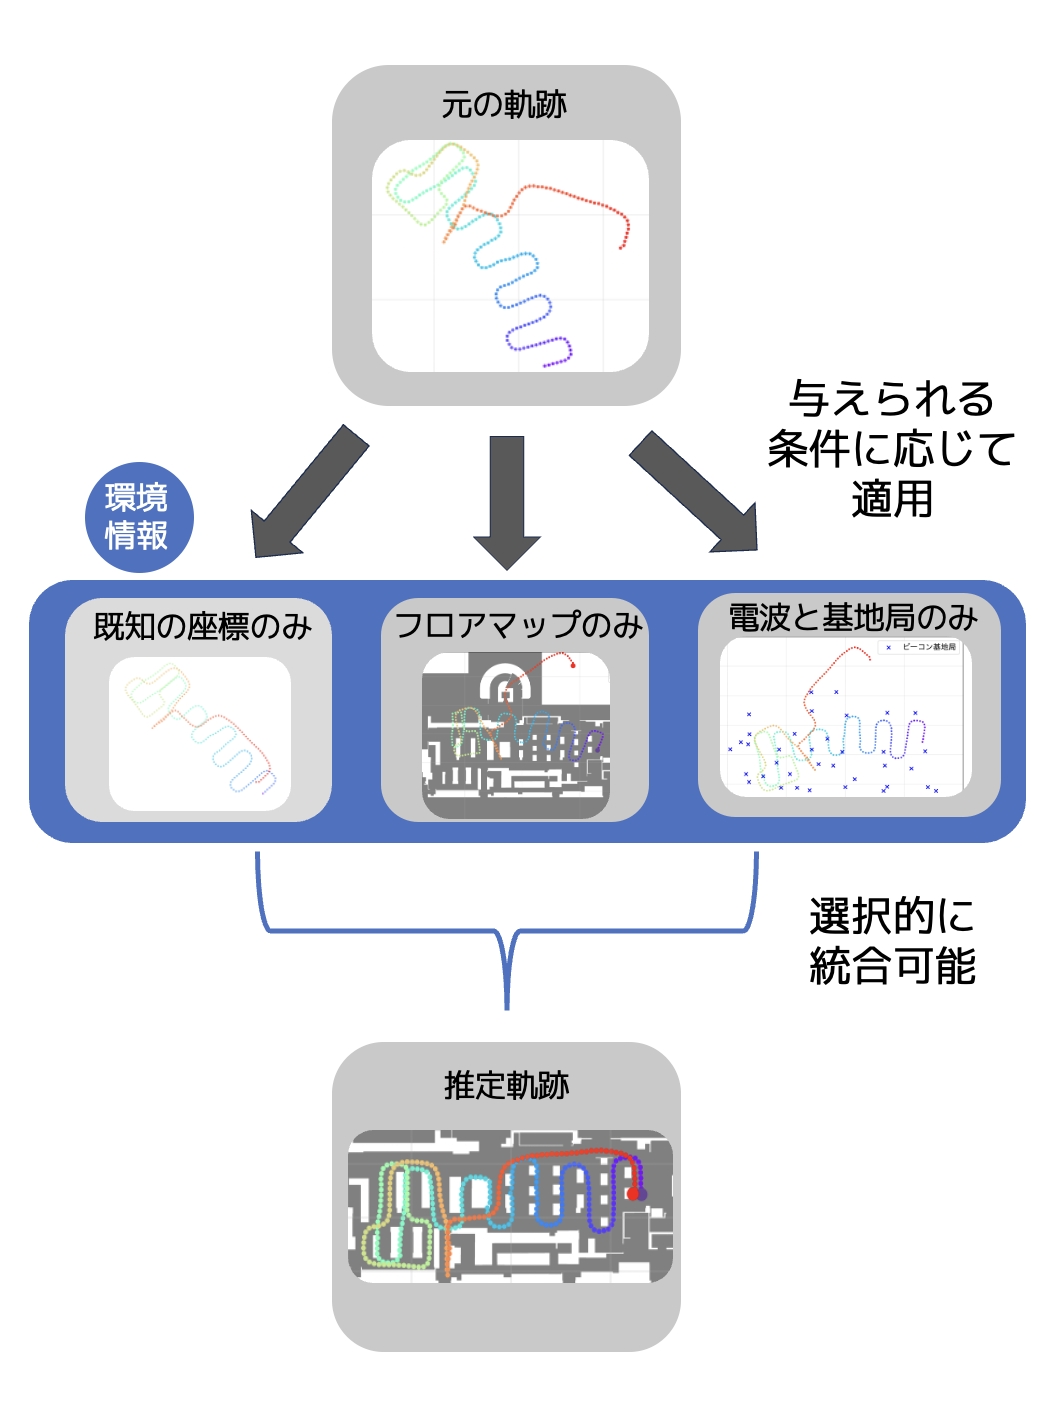
\includegraphics[width=\linewidth]{image/integrate11.png}
    \caption{環境条件に応じた補正の選択と適用}
    \label{fig:corrector-class}
\end{figure}


\subsection{気圧データを用いた3次元的な位置推定}
屋内環境における3次元的な位置推定において,歩行者の階層推定が必要である.
本ライブラリではスマートフォンの気圧センサから得られるデータを活用し,
PDRによる2次元軌跡に階層情報を付加する手法を実装している.

気圧データを用いた階層検知にはセンサのノイズや環境変化による問題がある.
これらに対処するため,本ライブラリでは安定区間検出とクラスタリングを組み合わせた2段階の方法を採用している.
まず気圧の変動が小さい安定区間を検出し,次にDBSCANアルゴリズムを適用して階層のグルーピングを行う.
また階層間の遷移は,2つの安定区間に挟まれた変動区間において顕著な気圧変化として検出される.
これにより商業施設やオフィスビルなど,複数階層を有する建物内での継続的な位置推定を実現する.



\section{評価と他環境での検討}

本章ではライブラリの基本性能をPDRベンチマーク標準化委員会が主催する評価環境で確認する.
また他環境での具体的な適用の検討を行う.


\subsection{xDR Challenge 2023 環境での評価}

本ライブラリの検証環境としてPDRベンチマーク標準化委員会が主催する
xDR Challenge 2023\footnote{産業技術総合研究所,https://unit.aist.go.jp/harc/xDR-Challenge-2023/(2023年10月)}
の環境を用いた.このコンペティションでは高速道路のサービスエリアを対象とし,
歩行時のスマートフォンからのセンサデータ,BLEビーコンからの受信電波強度,
LiDARからの正解位置情報の一部が提供される.
またフロアマップ情報,各ビーコンのフロアマップにおける基地局の位置情報も提供される.

xDR Challenge 2023では位置推定の精度を多角的に評価するため,円形誤差(l\_ce),局所空間における円形精度(l\_ca),
誤差蓄積勾配(l\_eag),速度誤差(l\_ve),障害物回避要件(l\_obstacle)の5つの指標を採用している.
本ライブラリの評価結果では,l\_ce(88.55点),l\_eag(93.02点),l\_ve(95.55点),l\_obstacle(93.48点)と
大半の指標で90点前後のスコアを達成した.
特に速度誤差と障害物回避要件で高いスコアを記録し,
基本的なPDRアルゴリズムとフロアマップの補正が効果的に機能しているのが示された.
一方局所空間における円形精度(l\_ca)は62.51点と低い結果となった.
これは実装アルゴリズムが比較的シンプルな構成であり,環境変化への対応力が限定的であるのを示唆している.

% TODO: 精度的には高い期待はできないものの最低限の適用する価値はあるみたいな文章が欲しい.

% TODO: 通過時刻を正確に記録できるから何感がある.それでどう活用できるか述べないといけない気がする.
\subsection{他環境での検討}
本ライブラリの他環境への適用可能性として,駅構内と大学キャンパスでの検討を行う.
駅構内では,改札の位置を利用したドリフト補正が適用できる.改札は固定位置であり,
ICカードの利用により通過時刻も正確に記録できる.
またフロアマップ情報の入手も比較的容易であり,マップマッチング補正の適用が期待できる.

大学キャンパスでは,Wi-Fiの基地局を活用した補正が有効である.
キャンパス内には基本的にWi-Fi基地局が存在しており,新規機器設置のコストを抑えられる.
ただし基地局の正確な位置情報の把握が困難な場合
フィンガープリントを用いた補正が適している場合がある.



\section{今後の課題}
PDRアルゴリズムの基本性能の向上は,引き続き課題である.
現状の実装では,歩行速度や路面状況の急激な変化に対する追従性に改善の余地がある.
より高度な手法として,パーティクルフィルターの導入を検討している.
これは複数の位置や方向の可能性を並行して評価できるため
環境の不確実性に対してよりロバストな位置推定が期待できる.
評価方法の拡充も重要であり,商業施設やオフィスビルなど,異なる特性を持つ環境での検証を進める必要がある.


\bibliographystyle{junsrt}
\bibliography{reference}

\end{document}


